\documentclass{svproc}
\usepackage[a4paper, bindingoffset=0.2in, 
			left=.7in, right=.7in,
			top=1in, bottom=1in,
			footskip=.25in]{geometry}
\setlength{\columnsep}{30pt}

\usepackage{url}
\usepackage{graphicx}
\usepackage[utf8]{inputenc}
\usepackage{float}
\usepackage{multicol}

\pagestyle{plain}

\graphicspath {{images/}}

\def\UrlFont{\rmfamily}

\begin{document}
	\mainmatter
	\title{SOFTWARE DESIGN FOR A ROBOT TO ASSIST LAPAROSCOPIC SURGERY}
	%
	\titlerunning{Software Design} 
	
	\author{Dayanne Fernandes}
	
	\institute{Robotics and Automation Laboratory (LARA), \\
		University of Brasilia, Brazil\\
		\email{dayannefernandesc@gmail.com}}
	
	\maketitle              
	
	\begin{abstract}
		
		\keywords{Software Design, Robotics, Laparoscopic Surgery, CLARA, Julius, QT, C++}
	\end{abstract}
	
	\begin{multicols}{2}
		
	\section{Introduction}
	
	% laparoscopic surgery
	
	In the beginning of 1980s, laparoscopic surgery was migrated from diagnostic to a surgical procedure. Semm K and Muehe E are the medics that introduced this technique for a wide field of indications, e.g., appendectomy, cholecystectomy, reflux surgery, gastric surgery, urology \cite{pmid26713285}. 
	
	% robots to aid laparoscopic surgery
	Nowadays the use of robotic surgery system are becoming more common, its benefits are being studied all around the world. Robotic technology allows the surgeon to increase dexterity and the degree of maneuverability to perform complex tasks in a minimally invasive fashion way \cite{doi:10.3109/10929088.2010.541620}. 
	
	% current robots to aid laparoscopic surgery 
	
 	Laparoscopic surgery demands an operating surgeon to make the medical procedure and a camera driver to show the surgeon the location of the operative field. This structure come with lots of problems, e.g. conflicts about the optimum visualization, fatigue of the assistant who holds the camera \cite{pmid28643066}, inaccurate movements, image tremors.
 	
 	There are many projects to solve the problems about the fatigue during laparoscopic surgery, e.g., EndoAssist \cite{pmid25484949}, Vicky \cite{pmid17867952}. These solutions are very expansive to apply to Brazilian's public health system (\textit{SUS}). In this context, CLARA is a low-cost project created at \textit{LARA} (Robotics and Automation Laboratory, University of Brasilia) to help the operating surgeon to procedure the surgery.
 	
 	% clara project 
 	
 	\textit{CLARA}'s project was designed to help the operating surgeon to perform the procedure with full control of the tools through effective interfaces, voice recognition and a joystick linked with the laparoscopic grasper. The voice control was compared with foot pedal interface, and they concluded that voice control was more accurate and had the advantage of not requiring the surgeon to look away from the operative field \cite{pmid16844449}. 
 	
 	% clara software and other softwares to aid biomedical robots (ros)
 	
 	The software was designed them to be applied into public hospitals. Compatibility, modularity, fault-tolerance, security, usability, performance and maintainability were topics considered during the software modeling process. This paper shows a software designed to assist laparoscopic robot surgery with all the aspects cited above.
 	
	\section{CLARA Structure}
	
	% mechanical
	
	% hardware
	
	% software
	
	\section{Software Design}
	
	% modules and qt
	An overview of CLARA software is illustrated at Figure~\ref{fig:clara}. \textit{Qt5}\cite{qt} is used as the main framework of the system. \textit{QT} is an open source (\textit{LGPLv3}\cite{lgpl}), cross-platform framework with a thread library that helps control the asynchronous modules and a GUI component to produce its visualization.
	
	\begin{figure}[H]
		\centering
		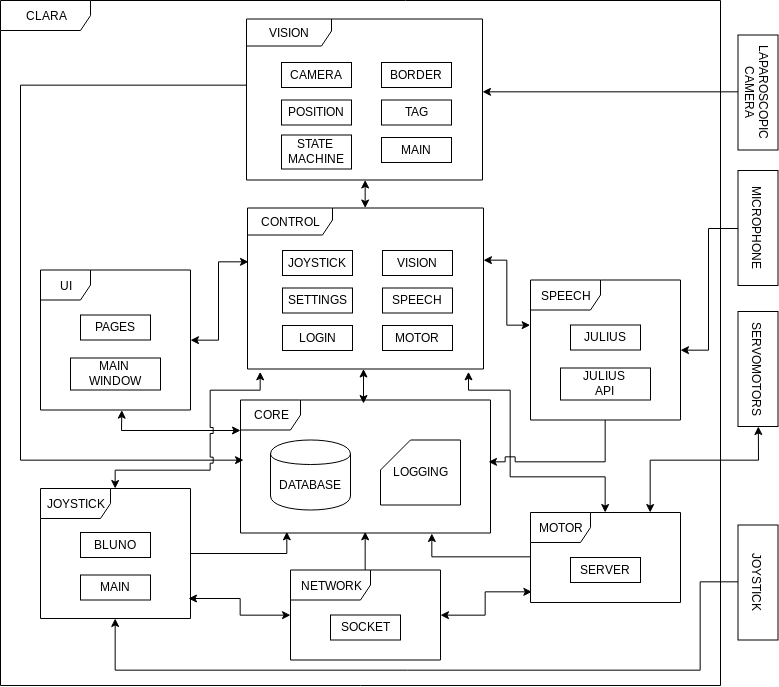
\includegraphics[width=0.45\textwidth]{clara.png}
		\caption{CLARA software design overview.}
		\label{fig:clara}
	\end{figure}
	
	\subsection{Core}
	
	% logging
	
	% database 
		
	\subsection{Network}
		
	\subsection{Speech}
	
	% julius
	\textit{Julius}\cite{lee2009recent} is a open-source (\textit{GPL}\cite{gpl}) speech recognition.
	
	\subsection{Vision}
	
	% opencv and boost
	This module is responsible to estimate the 2D pose of a single instrument tip\cite{vision} using \textit{OpenCV} and \textit{Boost}'s libraries.
	
	\subsection{Motor}
	
	\subsection{Joystick}
	
	\subsection{UI}
	
	The usability and user experience was put as a priority to produce \textit{CLARA}'s software. 
	
	% pages control
	
	\subsection{Test}
	
	\section{Conclusion}

	% Why the software design elaborated on CLARA project was important and efficient and effective
	Develop a software to be applied in a public hospital in Brazil demands a few worries, e.g. use cross-platforms frameworks since we don't know the operating system used on hospital machines, choose open source frameworks and libraries to help achieve the low-cost aim.
	
	% libraries used
	CLARA software covered all the attributes above using \textit{Julius} and \textit{QT} frameworks. 
	
	\section{Acknowledgements}
	
	CLARA project is funded by the Brazilian Ministry of Health (Term of Cooperation no 121/2013, Process 25000.169843/2013-83). 
		
	% ---- Bibliography ----
	\bibliographystyle{unsrt}
	\bibliography{article} 
	
	\end{multicols}
	
\end{document}
